% !TeX root = RJwrapper.tex
\title{corVis: An R Package for Visualising Associations and Conditional Associations}
\author{by Amit Chinwan and Catherine Hurley}

\maketitle

\abstract{%
We present \CRANpkg{corVis}, an R package for visualizing association and conditional association using measures of association. The package provides matrix and linear layout for displaying bivariate association possibly grouped by levels of a categorical variable, using measures suitable for numerical, ordinal and nominal variables. With these displays, an analyst can gain an overview about the interesting structure and underlying patterns in the data. We provide a detailed look at the package functions and discuss the implemented design choices. We also provide an illustration of the package on an example dataset.
}

\hypertarget{introduction}{%
\section{Introduction}\label{introduction}}

The first stage in data analysis includes exploring numerical and graphical variable summaries.
Correlation matrix displays are useful for showing bivariate associations. Generally these show Pearson's correlation, a measure of linear association for pairs of numerical variables. Alternative measures are needed to capture complex non-linear associations, and associations involving categorical variables.
In addition, correlation displays commonly use a matrix layout which require a lot of space for high-dimensional datasets.

In this paper, we introduce the R package \CRANpkg{corVis} which addresses the limitations of existing correlation matrix displays.
As most datasets are a mix of numerical, ordinal and categorical variables,
we provide association measures for pairs of numerical, ordinal and categorical variables. We also provide measures for mixed pairs of variables, where one variable is categorical and the other is numerical.
For numerical variables, we include measures of non-linear association such as distance correlation (Székely, Rizzo, and Bakirov 2007) and the maximal information coefficient (MIC) (Reshef et al. 2011){]}.
We provide a new tibble data structure for (possibly multiple) association measures for each pair of variables. The data structure is also used for pairwise association measures for levels of a grouping variable.

In \CRANpkg{corVis} the association measures are displayed using two different layouts. Our first display uses a matrix-layout, similar to existing correlation matrix displays. A novel feature is that our version can show multiple association measures for each pair of variables so that patterns other than linear association, or association that depends on the level of a grouping variable, become evident. For high-dimensional datasets, matrix layouts become unwieldy and run out of space, so our second display uses a linear layout, showing one or more association measures for each pair of variables. This is especially useful when the analyst wishes to limit the display to pairs of variables showing non-negligible associations.
Following Friendly (2002) who employed ordered correlation displays enabling quick identification of groups of variables with high mutual correlation, we use seriation for matrix displays and importance sorting for linear displays. In both cases the goal is to place highly-associated variables or variable pairs with high differences in prominent locations so they become easier to identify.

The next section provides a review of existing packages which deal with correlation displays and a background on association measures and the packages used for calculating them. Then we describe our approach to calculating the association measures, followed by illustrations of the proposed displays. We conclude with a discussion and future work.

\hypertarget{background}{%
\section{Background}\label{background}}

In this section, we provide a brief review of some of the association measures used in the package \CRANpkg{corVis} and the existing packages used for correlation displays.

\hypertarget{association-measures}{%
\subsection{Association Measures}\label{association-measures}}

An association measure is defined as a numerical summary quantifying the relationship between two or more variables. The measure is symmetric if its value is invariant to the order of inputs. For example, Pearson's correlation coefficient is a symmetric measure with a value in the range {[}−1,1{]} summarising the strength and direction of the linear relationship between two numeric variables. Similarly, Kendall's and Spearman's rank correlation coefficients are symmetric measures assessing monotonic association between numeric variables. This section starts with a review of the association measures for numeric pairs, followed by measures for nominal/ordinal pairs and then finally measures suitable for mixed variable pairs.

Because Pearson's correlation is a measure of linear dependence only, it misrepresents relationships that aren't linear and makes it a less useful measure. The recently developed measures such as distance correlation (Székely, Rizzo, and Bakirov 2007) and MIC (Reshef et al. 2011) overcome this limitation and are more suitable for datasets with both linear and non-linear patterns.

The distance correlation coefficient is a symmetric measure with its value in \([0,1]\) and summarizes any relationship between two numeric variables using the distances between observations of these variables. The distance correlation is \(0\) if and only if the variables are independent and \(1\) when the variables are perfectly linear. The R package \CRANpkg{energy} (Rizzo and Szekely 2022) implements distance correlation.

The maximal information coefficient (MIC) is an information theory measure which uses mutual information among the two variables for its calculation. The main idea is to find a grid out of possible grids on a scatterplot of two numeric variables, in order to discretize the variables, which maximises the mutual information. A normalisation technique is used to make the mutual information from different grids comparable. Referred to as `a correlation of 21st century' (Speed 2011), MIC is capable of summarizing different types of relationships, not just linear or monotonic, between numeric variables and is in the interval \([0,1]\). MIC is a symmetric measure where a zero value indicates independence among the variables and a value of 1 represents a noiseless functional relationship. Reshef et al. (2011) used MIC and other related statistics to explore pairwise relationships in large data sets such as major-league baseball, gene expression, global health, and the human gut microbiota. The MIC and related maximal information based non parametric exploration statistics have been implemented in the R package \CRANpkg{minerva} (Albanese et al. 2012).

Simon and Tibshirani (2014) simulated pairs of variables with different relationships at varying levels of noise and showed that distance correlation has more statistical power than MIC. Kinney and Atwal (2014) showed that MIC is not equitable and its values might not be affected by variable noise for certain relationships. They also note that MIC could have a value of 1.0 for differing noise levels.

The alternating conditional expectations (ACE) algorithm (Breiman and Friedman 1985) estimates optimal transformations between response and predictor variables during the regression analysis. For numeric variable pairs, the algorithm calculates the maximal correlation coefficient among the transformed variables and summarizes the non-linear relationship between them. It is a symmetric measure and takes a value in interval \([0,1]\). It is equal to zero if and only if the variables are independent. The R package \CRANpkg{acepack} (Spector et al. 2016) provides an implementation of ACE algorithm.

For nominal variable pairs, measures such as Pearson's contingency coefficient and Uncertainty coefficient (Theil 1970) are used to quantify the association. Pearson's contingency coefficient is a symmetric measure which uses the \({\chi}^2\) value from Pearson's \({\chi}^2\) test for independence and is scaled in the interval \([0,1]\). The uncertainty coefficient (Theil 1970) measures the proportion of uncertainty in one variable which is explained by the other. The uncertainty coefficient is in the range \([0,1]\) and is not symmetric. A symmetric version is used by taking the mean of the uncertainty coefficients obtained by treating each variable as an independent variable once. Both the measures have been provided in the R package \CRANpkg{DescTools} (Andri et mult. al. 2022).

Agresti (2010) provides an overview of the measures which are used for exploring the association between ordinal variables. Kendall's tau-b (Kendall 1945) is a measure of the strength and direction of the association between two ordinal variables. It is based on the number of concordances and discordances in paired observations of the variables and summarizes the association in the range \([-1,1]\). The polychoric correlation (Olsson 1979) measures the correlation between two ordinal variables by assuming two normally distributed latent variables and summarizes the association in \([-1,1]\). Both Kendall's tau-b and polychoric correlation are symmetric and are available in the R packages \CRANpkg{DescTools} (Andri et mult. al. 2022) and \CRANpkg{polycor} (Fox 2022).

Normalized mutual information (NMI) is a useful measure to summarise the association for mixed variable pairs. The package \CRANpkg{linkspotter} provides an implementation of Maximal Normalized Mutual Information for different variable pairs. The numeric variables are first discretized and then used for calculating mutual information. We use this measure for numeric, nominal and mixed pairs in \CRANpkg{corVis}. Canonical correlation is used to assess relationships for mixed variable pairs by converting nominal variables into sets of dummy variables, which are then assigned scores to find the maximal correlation. For two numeric variables, this measure is identical to absolute correlation, for two factors the correlation is identical to that obtained from correspondence analysis. We provide implementation of canonical correlation in \CRANpkg{corVis}.

In \CRANpkg{corVis}, we provide multiple association measures which can discover non-linear patterns and interesting associations featuring categorical variables.

\hypertarget{correlation-displays}{%
\subsection{Correlation Displays}\label{correlation-displays}}

According to Hills (1969), ``the first and sometimes only impression gained by looking at a large correlation matrix is its largeness''. To overcome this, Murdoch and Chow (1996) proposed a display for large correlation matrices which uses a matrix layout of ellipses where the parameters of the ellipses are scaled to the correlation values. Friendly (2002) expanded on this idea by rendering correlation values as shaded squares, bars, ellipses, or circular `pac-man' symbols.

\begin{table}

\caption{\label{tab:corrdisplay-packages}List of the R packages dealing with correlation or correlation displays with information on whether the plots display multiple measures, conditional display of measures and mixed variables in a single plot}
\centering
\begin{tabular}[t]{lll}
\toprule
Package & Display & MixedVariables\\
\midrule
corrplot & heatmap & \\
mbgraphic & heatmap & \\
corrr & heatmap/network & \\
corrgrapher & network & \\
linkspotter & network & Yes\\
\addlinespace
correlation & heatmap/network & \\
corVis & heatmap/matrix/linear & Yes\\
\bottomrule
\end{tabular}
\end{table}

Nowadays, there are many R packages devoted to correlation visualisation. Table \ref{tab:corrdisplay-packages} provides a summary, listing the displays offered, and whether these extend to factor variables or mixed numeric-factor pairs.

The R package \CRANpkg{corrplot} (Wei and Simko 2021) provides an implementation of the methods in Friendly (2002) and produces displays in a matrix layout. The package \CRANpkg{corrr} (Kuhn, Jackson, and Cimentada 2020) organises correlations as tidy data first, so leveraging the data manipulation and visualisation tools of the \CRANpkg{tidyverse} (Wickham et al. 2019), which then can be displayed in a matrix format. Friendly (2002) also focused on ordering of the variables for correlation displays where the variables were ordered using the angular ordering of the first two eigen vectors of the correlation matrix. The ordering places highly-correlated pairs of variables nearby, making it easier to quickly identify groups of variables with high mutual correlation. The package \CRANpkg{corrplot} (Wei and Simko 2021) provides various ordering techniques for matrix displays along with the method implemented in Friendly (2002). Grimm (2017) in the package \CRANpkg{mbgraphic} explored correlation structure of numeric variables using interactive matrix displays. She extended the display to general measures like scagnostics, which are measures characterizing a scatterplot, along with two more measures, based on smoothing splines and distance correlation.

The package \CRANpkg{corrgrapher} (Morgen and Biecek 2020) uses a network plot for exploring correlations, where the nodes close to each other have high correlation magnitude, edge thickness encodes the absolute correlation value and edge color indicates the sign of correlation. The package also handles mixed type variables by using association measures obtained as transformations of \(p\)-values obtained from Pearson's correlation test in the case of two numeric variables, Kruskal's test for numerical and factor variables, and a chi-squared test for two categorical variables. The package \CRANpkg{corrr} (Kuhn, Jackson, and Cimentada 2020) also offers network displays where line-thickness encodes correlation magnitude, with a filtering option to discard low-correlation edges. Another package for plotting correlations in a network layout is \CRANpkg{linkspotter} (Samba 2020) which offers a variety of association measures (distance correlation, MIC, maximum normalized mutual information) in addition to correlation, where the measure used depends on whether the variables are both numerical, categorical or mixed. The results are visualized in a network plot, which may be packaged into an interactive shiny application.

The R package \CRANpkg{correlationfunnel} offers a novel linear display which assists in feature selection in a setting with a single response and many predictor variables. All numeric variables including the response are binned. All (now categorical) variables in the resulting dataset are one-hot encoded and Pearson's correlation calculated with the response categories. The correlations are visualised in a dot-plot display, where predictors are ordered by maximum correlation magnitude. Correlations between one-hot encoded variables are challenging to interpret, especially as the number of levels increase. In corVis we offer a similar dot-plot display, but showing multiple correlation or association measures, or alternatively measures stratified by a grouping variable.

Our own package \CRANpkg{corVis} offers a variety of displays, and has new features not available elsewhere, in particular simultaneous display of multiple association measures, and association displays stratified by levels of a grouping variable. This will be described in the following sections.

\hypertarget{overview-of-corvis}{%
\section{\texorpdfstring{Overview of \texttt{corVis}}{Overview of corVis}}\label{overview-of-corvis}}

The R package \CRANpkg{corVis} offers a flexible framework to investigate and visualise associations using measures of association, in datasets with mixed variable types. The calculation and visualisation of association measures are carried out separately in \CRANpkg{corVis}, making it an open-ended package for both data structure and display of association measures. This allows users to leverage the widely used \CRANpkg{tidyverse} and \CRANpkg{ggplot2} framework for exploring these data structures.

In\CRANpkg{corVis}, we extend existing correlation displays beyond numeric variables by including mixed variable types and propose displays for multiple association measures useful for uncovering non-linear patterns or associations depending on the levels of a grouping variable. While designing these displays we consider matrix and linear layouts. Linear layouts are useful for high-dimensional datasets and allow a user to limit the display to variable pairs showing strong associations. We also order these displays so that the variable pairs with a strong association or a high difference in measures are placed at prominent positions.

\begin{table}

\caption{\label{tab:function-corVis}List of functions in corVis package}
\centering
\begin{tabular}[t]{>{}lll}
\toprule
Function & Usage & Description\\
\midrule
\textbf{calc\_assoc} & Calculation & Calculates association measures\\
\textbf{calc\_assoc\_all} & Calculation & Calculates all the association measures available in package\\
\textbf{plot\_assoc\_matrix} & Visualization & Visualize assocition and conditional association in matrix plot\\
\textbf{plot\_assoc\_linear} & Visualization & Visualize assocition and conditional association in linear plot\\
\textbf{show\_assoc} & Visualization & Association (or conditional) plot for a pair of variables\\
\bottomrule
\end{tabular}
\end{table}

Table \ref{tab:function-corVis} provides a list of the functions available in the package. The functions \texttt{calc\_assoc} and \texttt{calc\_assoc\_all} are responsible for calculating association measures which are used as input for the \texttt{plot\_assoc\_matrix} and \texttt{plot\_assoc\_linear} functions. The functions \texttt{plot\_assoc\_matrix} and \texttt{plot\_assoc\_linear} produces association display, multiple association measures display and conditional association display, in a matrix and linear layout respectively. We provide detailed examples on calculation and visualisation of association and conditional association in next sections.

\hypertarget{example-data}{%
\subsection{Example: Data}\label{example-data}}

We use the Daily Bike Sharing dataset (Fanaee-T and Gama 2014) from the R package \CRANpkg{timetk} (Dancho and Vaughan 2022) which contains daily count of rental bike transactions between years 2011 and 2012 in Capital bikeshare system. The dataset also includes corresponding daily weather information such as humidity, temperature and windspeed, and seasonal information such as season, whether the day is a holiday and whether the day is a working day.

\begin{table}

\caption{\label{tab:bikedata}Variable description of the Daily Bike Sharing dataset}
\centering
\resizebox{\linewidth}{!}{
\begin{tabular}[t]{lll}
\toprule
Variable & Description & VariableType\\
\midrule
dteday & date & date\\
season & season with categories Winter, Spring, Summer and Fall & nominal\\
yr & year of day with categories 2011 and 2012 & nominal\\
mnth & month of day with months as categories & nominal\\
holiday & whether day is a holiday or not & nominal\\
\addlinespace
weekday & day of the week & nominal\\
workingday & if day is neither weekend nor holiday it is Yes, otherwise is No & nominal\\
weathersit & weather situation of the day with categories clear, cloudy, lightP & nominal\\
temp & normalized temperature in Celsius & numeric\\
atemp & normalized feeling temperature in Celsius & numeric\\
\addlinespace
hum & normalized humidity & numeric\\
windspeed & normalized windspeed & numeric\\
casual & count of casual users & numeric\\
registered & count of registered users & numeric\\
cnt & count of total rental bikes including both casual and registered & numeric\\
\bottomrule
\end{tabular}}
\end{table}

Table \ref{tab:bikedata} provides a brief description of Daily Bike Sharing data along with the types of variables present in the dataset. We use the dataset throughout this paper for illustrative usage of the package.

\hypertarget{data-structures}{%
\subsection{Data Structures}\label{data-structures}}

We provide three tidy data structures which are explored using functions in \CRANpkg{corVis} or can be manipulated or visualized by leveraging tools in \CRANpkg{tidyverse} These data structures are: \texttt{pairwise}, \texttt{multi\_pairwise} and \texttt{cond\_pairwise}. Here, we provide an example of these three data structures along with how they are beneficial when used in the \CRANpkg{tidyverse} environment.

The \texttt{pairwise} data structure is a data format which contains scores for pairs of variables in a dataset for which a specified measure is defined. For example, the function \texttt{tbl\_dcor} calculates the distance correlation measure for every numeric variable pair in the dataset. Each row of the \texttt{pairwise} object is characterized by the variable pair and association measure type.

\begin{verbatim}
# a subset of bike dataset
bike_s <- bike |> 
  dplyr::select(temp, windspeed, registered,weathersit, workingday)
dcor_bike <- tbl_dcor(bike_s)
dcor_bike
\end{verbatim}

\begin{verbatim}
#> # A tibble: 3 x 5
#>   x          y         measure measure_type pair_type
#>   <chr>      <chr>       <dbl> <chr>        <chr>    
#> 1 windspeed  temp        0.181 dcor         nn       
#> 2 registered temp        0.531 dcor         nn       
#> 3 registered windspeed   0.208 dcor         nn
\end{verbatim}

\begin{verbatim}
class(dcor_bike)
\end{verbatim}

\begin{verbatim}
#> [1] "pairwise"   "tbl_df"     "tbl"        "data.frame"
\end{verbatim}

We define a \texttt{multi\_pairwise} data structure as a data format which consists of multiple scores for variable pairs in the dataset. Similar to the \texttt{pairwise} object, every row of the \texttt{multi\_pairwise} object is defined by the variable pair and measure type. An analyst interested in finding how different the association measure values are for each pair can use this object with \CRANpkg{tidyverse} tools to find the range of measures.

\begin{verbatim}
multi_bike <- calc_assoc_all(bike_s,
                                 c("pearson","nmi","ace","uncertainty"))
class(multi_bike)
\end{verbatim}

\begin{verbatim}
#> [1] "multi_pairwise" "pairwise"       "tbl_df"         "tbl"           
#> [5] "data.frame"
\end{verbatim}

\begin{verbatim}
# calculating range of measures
multi_bike |> 
  group_by(x,y) |>
  summarise(range=max(measure)-min(measure),.groups = "drop") |>
  arrange(desc(range))
\end{verbatim}

\begin{verbatim}
#> # A tibble: 10 x 3
#>    x          y           range
#>    <chr>      <chr>       <dbl>
#>  1 registered windspeed  0.458 
#>  2 windspeed  temp       0.415 
#>  3 registered temp       0.374 
#>  4 weathersit registered 0.278 
#>  5 workingday registered 0.188 
#>  6 weathersit temp       0.137 
#>  7 weathersit windspeed  0.115 
#>  8 workingday weathersit 0.0585
#>  9 workingday windspeed  0.0409
#> 10 workingday temp       0.0194
\end{verbatim}

The final data structure in \CRANpkg{corVis} is \texttt{cond\_pairwise} which contains scores for every variable pair at different levels of a conditioning variable. In this case, each row is uniquely identified by a variable pair and a level of the conditioning variable. For exploring pairwise differences in groups, an analyst can easily use data manipulation tools available in \CRANpkg{tidyverse} ecosystem.

\begin{verbatim}
cond_bike <- calc_assoc(bike_s,
                            by="weathersit")
class(cond_bike)
\end{verbatim}

\begin{verbatim}
#> [1] "cond_pairwise" "pairwise"      "tbl_df"        "tbl"          
#> [5] "data.frame"
\end{verbatim}

\begin{verbatim}
# calculating difference in the group
cond_bike |> 
  group_by(x,y) |>
  summarise(diff=max(measure)-min(measure),.groups = "drop") |>
  arrange(desc(diff))
\end{verbatim}

\begin{verbatim}
#> # A tibble: 6 x 3
#>   x          y            diff
#>   <chr>      <chr>       <dbl>
#> 1 registered windspeed  0.421 
#> 2 workingday windspeed  0.411 
#> 3 windspeed  temp       0.385 
#> 4 workingday registered 0.294 
#> 5 workingday temp       0.205 
#> 6 registered temp       0.0777
\end{verbatim}

It is worth noting that both \texttt{multi\_pairwise} and \texttt{cond\_pairwise} objects inherit the \texttt{pairwise} class and satisfies the definition of the \texttt{pairwise} data structure.

\hypertarget{corvis-calculating-association-measures}{%
\section{corVis: Calculating Association Measures}\label{corvis-calculating-association-measures}}

For exploring associations using \CRANpkg{corVis}, the first step is to calculate association measures for variable pairs in a dataset. Table \ref{tab:association-measures} lists the functions provided in the package to calculate measures of association along with the information on the type of variable pairs they can be applied with. It also includes details about the external package functions used to calculate and the range for these measures. The association measures available in \CRANpkg{corVis} are symmetric. We convert asymmetric measures to symmetric ones by taking either the mean or the maximum of the measures calculated by treating each variable from the pair as an independent variable. The functions \texttt{tbl\_ace} and \texttt{tbl\_cancor} which calculate the maximal correlation coefficient among the transformed variables and canonical correlation respectively have been implemented in \CRANpkg{corVis}.

\begin{table}

\caption{\label{tab:association-measures}List of the functions available in the package for calculating different association measures along with the packages used for calculation.}
\centering
\resizebox{\linewidth}{!}{
\begin{tabular}[t]{lllllll}
\toprule
name & nn & ff & oo & nf & from & range\\
\midrule
tbl\_cor & y &  &  &  & stats::cor & {}[-1,1]\\
tbl\_dcor & y &  &  &  & energy::dcor2d & {}[0,1]\\
tbl\_mine & y &  &  &  & minerva::mine & {}[0,1]\\
tbl\_ace & y & y &  & y & corVis & {}[0,1]\\
tbl\_cancor & y & y &  & y & corVis & {}[0,1]\\
\addlinespace
tbl\_nmi & y & y &  & y & linkspotter::maxNMI & {}[0,1]\\
tbl\_polycor &  &  & y &  & polycor::polychor & {}[-1,1]\\
tbl\_tau &  &  & y &  & DescTools::KendalTauA,B,C,W & {}[-1,1]\\
tbl\_gkGamma &  &  & y &  & DescTools::GoodmanKruskalGamma & {}[-1,1]\\
tbl\_gkTau &  &  & y &  & DescTools::GoodmanKruskalTau & {}[0,1]\\
\addlinespace
tbl\_uncertainty &  & y &  &  & DescTools::UncertCoef & {}[0,1]\\
tbl\_chi &  & y &  &  & DescTools::ContCoef & {}[0,1]\\
\bottomrule
\end{tabular}}
\end{table}

The functions listed in Table \ref{tab:association-measures} for calculating association measures provide functionality for handling missing values or \texttt{NA} in the dataset. Each of these functions either has a \texttt{handle.na} argument or automatically uses pairwise complete observations (depending on the package used for calculation) for taking care of missing values present in the data. In \CRANpkg{corVis}, we do not handle date times, or circular variables (usually time-related). The only association measure which handles circular variables is ace, but we are not so far using this feature. In the bike data, the circular variables are \texttt{season}, \texttt{month} and \texttt{weekday}.

The \texttt{tbl\_*} functions require a dataset as an input and return a \texttt{pairwise} data structure. The output includes the pairs of variables for which the \texttt{tbl\_*} function is defined, the type of association measure, measure value and the type of variable pair. Our display functions \texttt{plot\_assoc\_matrix} or \texttt{plot\_assoc\_linear} can be used to plot this output in a matrix or linear layout respectively.

\hypertarget{calculating-association-measures-for-whole-dataset}{%
\subsection{Calculating association measures for whole dataset}\label{calculating-association-measures-for-whole-dataset}}

The \texttt{calc\_assoc} function calculates association measures for every variable pair in a dataset. The variable pairs in the output are unique pairs where \texttt{x} \(\neq\) \texttt{y}. Because of the tidy structure of the output, the data manipulation and visualization tools of \CRANpkg{tidyverse} (Wickham et al. 2019) are applicable and useful for further exploration of pairwise associations. The output of \texttt{calc\_assoc} is a \texttt{pairwise} data structure with one measure for each pair of variables in the dataset.

The code snippet below shows the calculation of association measures for a subset of the bike sharing data. We select three numeric (\texttt{temp}, \texttt{windspeed}, \texttt{registered}) and two nominal variables (\texttt{weathersit}, \texttt{workingday}) from the original dataset to demonstrate the usage of \texttt{calc\_assoc}. We include all of the function arguments for the below example and describe how these are useful. The inputs such as \texttt{by} and \texttt{include.overall} will be described in the section {[}Calculating conditional association{]}.

\begin{verbatim}
bike_s <- bike |> 
  dplyr::select(temp, windspeed, registered,weathersit, workingday)
bike_s_assoc <- calc_assoc(d = bike_s,
                           by = NULL,
                           types = default_assoc(),
                           include.overall = NULL,
                           handle.na = TRUE,
                           coerce_types = NULL)
bike_s_assoc
\end{verbatim}

\begin{verbatim}
#> # A tibble: 10 x 5
#>    x          y          measure measure_type pair_type
#>    <chr>      <chr>        <dbl> <chr>        <chr>    
#>  1 windspeed  temp       -0.158  pearson      nn       
#>  2 registered temp        0.540  pearson      nn       
#>  3 weathersit temp        0.121  cancor       nf       
#>  4 workingday temp        0.0527 cancor       nf       
#>  5 registered windspeed  -0.217  pearson      nn       
#>  6 weathersit windspeed   0.120  cancor       nf       
#>  7 workingday windspeed   0.0188 cancor       nf       
#>  8 weathersit registered  0.282  cancor       nf       
#>  9 workingday registered  0.304  cancor       nf       
#> 10 workingday weathersit  0.0613 cancor       ff
\end{verbatim}

\texttt{calc\_assoc} uses \texttt{tbl\_*} functions to calculate a measure for every variable pair. The \texttt{types} argument is a tibble of the \texttt{tbl\_*} functions for different types of variable pairs. The default is \texttt{default\_assoc()} which includes \texttt{tbl\_cor} if both the variables are numeric and calculate Pearson's correlation, \texttt{tbl\_gkGamma} if both the variables are ordinal and compute Goodman and Kruskal's gamma and \texttt{tbl\_cancor} for a factor pair and mixed pair and calculate the canonical correlation.

\begin{verbatim}
default_measures <- default_assoc()
default_measures
\end{verbatim}

\begin{verbatim}
#> # A tibble: 4 x 4
#>   funName     typeX   typeY   argList
#>   <chr>       <chr>   <chr>   <list> 
#> 1 tbl_cor     numeric numeric <NULL> 
#> 2 tbl_gkGamma ordered ordered <NULL> 
#> 3 tbl_cancor  factor  factor  <NULL> 
#> 4 tbl_cancor  factor  numeric <NULL>
\end{verbatim}

The default association measures are updated using the \texttt{update\_assoc} function. For example, an analyst interested in calculating Spearman's rank correlation for numeric pairs, ace measure for mixed pairs and nmi measure for factor pairs can update these measures as shown in the below code segment.

\begin{verbatim}
updated_assoc <- update_assoc(default_measures,
                              num_pair = "tbl_cor",
                              num_pair_argList = "spearman",
                              mixed_pair = "tbl_ace",
                              factor_pair = "tbl_nmi")
updated_assoc
\end{verbatim}

\begin{verbatim}
#> # A tibble: 4 x 4
#>   funName    typeX   typeY   argList  
#>   <chr>      <chr>   <chr>   <list>   
#> 1 tbl_cor    numeric numeric <chr [1]>
#> 2 tbl_nmi    ordered ordered <NULL>   
#> 3 tbl_cancor factor  factor  <NULL>   
#> 4 tbl_ace    factor  numeric <NULL>
\end{verbatim}

\begin{verbatim}
updated_bike_s_assoc <- calc_assoc(d = bike_s, 
                                 types = updated_assoc)
updated_bike_s_assoc
\end{verbatim}

\begin{verbatim}
#> # A tibble: 10 x 5
#>    x          y          measure measure_type pair_type
#>    <chr>      <chr>        <dbl> <chr>        <chr>    
#>  1 windspeed  temp       -0.147  spearman     nn       
#>  2 registered temp        0.531  spearman     nn       
#>  3 weathersit temp        0.189  ace          nf       
#>  4 workingday temp        0.0560 ace          nf       
#>  5 registered windspeed  -0.203  spearman     nn       
#>  6 weathersit windspeed   0.143  ace          nf       
#>  7 workingday windspeed   0.0568 ace          nf       
#>  8 weathersit registered  0.329  ace          nf       
#>  9 workingday registered  0.357  ace          nf       
#> 10 workingday weathersit  0.0613 cancor       ff
\end{verbatim}

The input \texttt{handle.na} for \texttt{calc\_assoc} manages the \texttt{NA} or missing value in the data. The default value is set to \texttt{TRUE} for using pairwise complete observations for calculating a measure of association between two variables.

Sometimes an analyst might want to treat a factor as an ordered variable. This will also be useful for pairs of binary variables where it will then be possible to see the direction of association. Alternatively, binary variables are treated as numerical. The input \texttt{coerce\_types} is used to convert variable types. The code segment below demonstrates how nominal factors can be converted into ordinal.

\begin{verbatim}
bike_s_assoc <- calc_assoc(d = bike_s,
                           by = NULL,
                           types = default_assoc(),
                           include.overall = NULL,
                           handle.na = TRUE,
                           coerce_types = list(ordinal=c("workingday", "weathersit")))
bike_s_assoc
\end{verbatim}

\begin{verbatim}
#> # A tibble: 10 x 5
#>    x          y          measure measure_type pair_type
#>    <chr>      <chr>        <dbl> <chr>        <chr>    
#>  1 windspeed  temp       -0.158  pearson      nn       
#>  2 registered temp        0.540  pearson      nn       
#>  3 weathersit temp        0.121  cancor       nf       
#>  4 workingday temp        0.0527 cancor       nf       
#>  5 registered windspeed  -0.217  pearson      nn       
#>  6 weathersit windspeed   0.120  cancor       nf       
#>  7 workingday windspeed   0.0188 cancor       nf       
#>  8 weathersit registered  0.282  cancor       nf       
#>  9 workingday registered  0.304  cancor       nf       
#> 10 workingday weathersit  0.133  gkGamma      oo
\end{verbatim}

\hypertarget{calculating-conditional-association-measures}{%
\subsection{Calculating conditional association measures}\label{calculating-conditional-association-measures}}

The function \texttt{calc\_assoc} is also used to calculate association measures for all the variable pairs at different levels of a categorical variable. This is useful in exploring the conditional associations and finding out variable pairs showing different associations at different levels of the grouping variable. The function has a \texttt{by} argument which is used as the grouping variable and needs to be categorical. The tibble output in the conditional setting has a similar structure as \texttt{calc\_assoc} with an additional \texttt{by} column representing the levels of the categorical variable. The output data structure has a \texttt{cond\_pairwise} class attribute which is used for displaying conditional measures. The data structure is also suitable for tidy operations with tools available in \CRANpkg{tidyverse} (Wickham et al. 2019).

\begin{verbatim}
bike_s_assoc_by <- calc_assoc(d = bike_s,
                            by = "workingday",
                            include.overall = TRUE)
bike_s_assoc_by
\end{verbatim}

\begin{verbatim}
#> # A tibble: 18 x 6
#>    x          y          measure measure_type by      pair_type
#>    <chr>      <chr>        <dbl> <chr>        <fct>   <chr>    
#>  1 windspeed  temp       -0.198  pearson      No      nn       
#>  2 registered temp        0.564  pearson      No      nn       
#>  3 weathersit temp        0.108  cancor       No      nf       
#>  4 registered windspeed  -0.259  pearson      No      nn       
#>  5 weathersit windspeed   0.228  cancor       No      nf       
#>  6 weathersit registered  0.214  cancor       No      nf       
#>  7 windspeed  temp       -0.137  pearson      Yes     nn       
#>  8 registered temp        0.550  pearson      Yes     nn       
#>  9 weathersit temp        0.136  cancor       Yes     nf       
#> 10 registered windspeed  -0.210  pearson      Yes     nn       
#> 11 weathersit windspeed   0.0795 cancor       Yes     nf       
#> 12 weathersit registered  0.349  cancor       Yes     nf       
#> 13 windspeed  temp       -0.158  pearson      overall nn       
#> 14 registered temp        0.540  pearson      overall nn       
#> 15 weathersit temp        0.121  cancor       overall nf       
#> 16 registered windspeed  -0.217  pearson      overall nn       
#> 17 weathersit windspeed   0.120  cancor       overall nf       
#> 18 weathersit registered  0.282  cancor       overall nf
\end{verbatim}

By default, the function \texttt{calc\_assoc} calculates the association measures for all the variable pairs at different levels of the grouping variable and the pairwise association measures for the ungrouped data (\texttt{overall}) when used with the \texttt{by} argument. This behavior can be changed by setting the \texttt{include.overall} argument to \texttt{FALSE}.

\begin{verbatim}
bike_s_assoc_by <- calc_assoc(d = bike_s,
                            by = "workingday",
                            include.overall = FALSE)
bike_s_assoc_by
\end{verbatim}

\begin{verbatim}
#> # A tibble: 12 x 6
#>    x          y          measure measure_type by    pair_type
#>    <chr>      <chr>        <dbl> <chr>        <fct> <chr>    
#>  1 windspeed  temp       -0.198  pearson      No    nn       
#>  2 registered temp        0.564  pearson      No    nn       
#>  3 weathersit temp        0.108  cancor       No    nf       
#>  4 registered windspeed  -0.259  pearson      No    nn       
#>  5 weathersit windspeed   0.228  cancor       No    nf       
#>  6 weathersit registered  0.214  cancor       No    nf       
#>  7 windspeed  temp       -0.137  pearson      Yes   nn       
#>  8 registered temp        0.550  pearson      Yes   nn       
#>  9 weathersit temp        0.136  cancor       Yes   nf       
#> 10 registered windspeed  -0.210  pearson      Yes   nn       
#> 11 weathersit windspeed   0.0795 cancor       Yes   nf       
#> 12 weathersit registered  0.349  cancor       Yes   nf
\end{verbatim}

\hypertarget{calculating-multiple-association-measures}{%
\subsection{Calculating multiple association measures}\label{calculating-multiple-association-measures}}

The comparison of multiple association measures help discover patterns other than linear. We calculate multiple measures with \texttt{calc\_assoc\_all} function in the package. The function takes a dataset and a vector of measures as input and outputs a tibble structure with multiple measures of association for every variable pair. The data structure has \texttt{multi\_pairwise} class attribute which is used for plotting multiple measure displays in matrix and linear layouts. The code section below calculates \texttt{pearson}, \texttt{dcor} and \texttt{cancor} measures for the variable pairs in subset of bike sharing data. The pairs for which a measure is not defined is not included in the result.

\begin{verbatim}
#> # A tibble: 38 x 5
#>    x          y          measure measure_type pair_type
#>    <chr>      <chr>        <dbl> <chr>        <chr>    
#>  1 windspeed  temp        0.158  cancor       nn       
#>  2 registered temp        0.540  cancor       nn       
#>  3 weathersit temp        0.121  cancor       nf       
#>  4 workingday temp        0.0527 cancor       nf       
#>  5 registered windspeed   0.217  cancor       nn       
#>  6 weathersit windspeed   0.120  cancor       nf       
#>  7 workingday windspeed   0.0188 cancor       nf       
#>  8 weathersit registered  0.282  cancor       nf       
#>  9 workingday registered  0.304  cancor       nf       
#> 10 workingday weathersit  0.0613 cancor       ff       
#> # ... with 28 more rows
\end{verbatim}

\hypertarget{corvis-visualising-association-measures}{%
\section{corVis: Visualising Association Measures}\label{corvis-visualising-association-measures}}

This section provides a detailed description of the novel displays proposed in the package \CRANpkg{corVis}. These displays show multiple association measures to identify variable pairs with non-linear patterns or pairs of variables showing different patterns at different levels of a grouping variable. The package includes functions \texttt{plot\_assoc\_matrix} and \texttt{plot\_assoc\_linear} to produce these displays in a matrix and linear layout respectively. In addition, the package also provides a function \texttt{show\_assoc} for a quick graphical overview of the relationship between two variables. It displays a scatterplot for numeric pairs, a bar plot for ordered and factor pairs, and a box plot for mixed variable pairs.

\hypertarget{matrix-displays}{%
\subsection{Matrix Displays}\label{matrix-displays}}

Conventionally, correlations have been displayed using a matrix layout. Matrix displays assist in analysing the multivariate structure between the variables. In \CRANpkg{corVis}, the \texttt{plot\_assoc\_matrix} function constructs a plot in the matrix layout displaying variable associations.

Careful ordering of matrix displays makes it easier to identify patterns and structures. Some examples include Friendly (2002) who demonstrated ordered correlation displays so that groups of variables with high mutual correlation are easily identified and hurley2004clustering who ordered variables in a scatterplot matrix so that interesting panels were positioned close to the main diagonal. They illustrate how seriation, a term to describe the ordering of objects, is useful to reveal interesting patterns. In \CRANpkg{corVis}, we use seriation methods from \CRANpkg{DendSer} (Hurley and Earle 2022) package to seriate matrix displays. In many of the seriation algorithms for matrix displays, the first step is to produce a dissimilarity or similarity matrix of objects to be clustered. Here, objects are the variables of a dataset. We use the Lazy path length (LPL) cost function proposed in \CRANpkg{DendSer} to obtain an ordering using the dissimilarity matrix of variables. This method is efficient in making interesting pairs more prominent in matrix displays by placing them at the start and top-left position.

We now illustrate the use of the \texttt{plot\_assoc\_matrix} function with \texttt{pairwise}, \texttt{multi\_pairwise} and \texttt{cond\_pairwise} data structures.

\hypertarget{association-measures-plot}{%
\subsubsection{Association Measures Plot}\label{association-measures-plot}}

For an association measure display, we start with calculating the default association measures for the bike sharing data (we drop variables dteday, weekday, atemp and cnt) using \texttt{calc\_assoc} and then plot the \texttt{pairwise} output using \texttt{plot\_assoc\_matrix} in a matrix layout.

\begin{verbatim}
bike$dteday <- NULL 
bike$weekday <- NULL
bike$atemp <- NULL
bike$cnt <- NULL

bike_assoc <- calc_assoc(d = bike)
plot_assoc_matrix(lassoc = bike_assoc,var_order = names(bike)) #default ordering
plot_assoc_matrix(lassoc = bike_assoc, var_order = "default") # DendSer ordering
\end{verbatim}

\begin{figure}
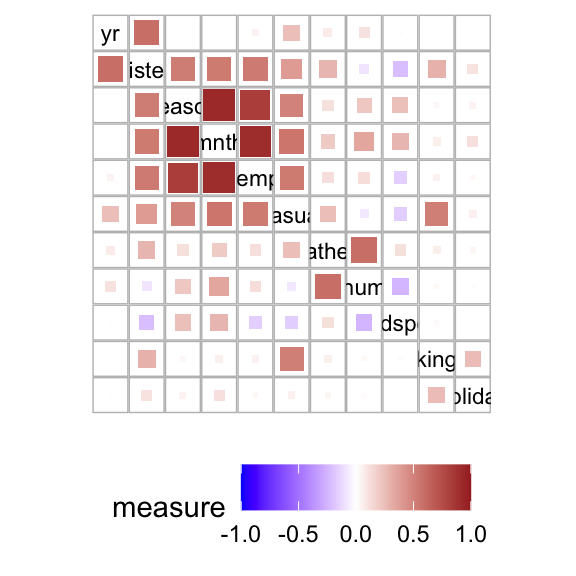
\includegraphics[width=0.5\linewidth]{rj-paper_files/figure-latex/assoc-matrix-bike-1} \includegraphics[width=0.5\linewidth]{rj-paper_files/figure-latex/assoc-matrix-bike-2} \caption{Left: variables in default order of the data; Right: variables ordered by LPL cost function. Association measures displays for bike sharing data showing Pearson's correlation for the numeric pairs, Goodman Kruskal's gamma measure for ordered pairs and canonical correlation for factor pairs and mixed pairs. The off diagonal cells show the measure value for a variable pair using a circle glyph. The color of every circle is mapped with the measure value for the pair and the radius of the circle is mapped to absolute measure value for the corresponding variable pair. It is easier to identify pairs on the right-hand plot with strong association, for example (casual, temp), (registered,yr) and (weathersit,hum). Also, there is a negative association for (windspeed,registered) suggesting the number of registered users decreased during windy days.}\label{fig:assoc-matrix-bike}
\end{figure}

The argument \texttt{var\_order} is used for ordering the variables. For ordering \texttt{pairwise} object, a dissimilarity matrix is constructed first where the dissimilarity is measured by \(-|m_{ij}|\), where \(m_{ij}\) is the association measure value for a variable pair \((i,j)\). This is followed by hierarchical clustering using the seriation weights (similar to the dissimilarity measure), which produces an order such that the LPL cost function is minimised. A user can also supply their own ordering perhaps obtained from other algorithms by specifying the \texttt{var\_order} argument.

Figure \ref{fig:assoc-matrix-bike} compares the default ordering of the variables in the dataset with ordering obtained by seriation using LPL cost function. The plot shows Pearson's correlation for the numeric pairs, Goodman Kruskal's gamma measure for ordered pairs and canonical correlation for factor pairs and mixed pairs. The plot on the right shows highly associated variables at the top left corner or along the diagonal of the display, making it easier for an analyst to identify associated pairs instantly.

The diagonal cells represent the variables present in the data. Every off diagonal cell contains a glyph, circle in this plot, which is filled with a divergent color scale representing the value of corresponding association measure for a variable pair. The \texttt{glyph} argument can be either \texttt{circle} or \texttt{square} and is only used for object with \texttt{pairwise} class. The radius of the circle is mapped to absolute value of the association measure. The argument \texttt{limits} specify the range of measure values to be mapped to colors. The default value is in the range \([-1,1]\).

Figure \ref{fig:assoc-matrix-bike} presents the novel feature of our display showing all the variables of a dataset in the same plot compared to corrgram which only shows association between numeric pairs. With canonical correlation as association measure for factor pairs or mixed pairs, we can observe from Figure \ref{fig:assoc-matrix-bike} that pairs such as (weathersit, humidity), (workingday, registered), (yr,casual), (season, casual) and (season, registered) are strongly associated.

In some cases, an analyst might want to handle some factors as ordinals to see the direction of association. As discussed in the previous section, we can convert variable types by specifying the \texttt{coerce\_types} argument. The code below shows an implementation and produces a display with some factor variables as ordinals.

\begin{verbatim}
bike_assoc_o <- calc_assoc(bike, 
                           coerce_types=list(ordinal=c("workingday", 
                                                       "yr", 
                                                       "weathersit", 
                                                       "holiday")))

plot_assoc_matrix(bike_assoc_o,
                  glyph="circle")
\end{verbatim}

\begin{figure}

{\centering \includegraphics{rj-paper_files/figure-latex/coerce-types-display-1} 

}

\caption{Association matrix display for bike sharing data showing Pearson's correlation for the numeric pairs, Goodman Kruskal's gamma measure for ordered pairs, canonical correlation for factor pairs and mixed pairs. The color of every circle is mapped with the measure value for the pair and the area of the circle is mapped by absolute measure value for the corresponding variable pair. The variables workingday, yr, weathersit and holiday have been converted to ordinals. The plot shows a strong negative association for (workingday, holiday) because no holiday is a working day.}\label{fig:coerce-types-display}
\end{figure}

Figure \ref{fig:coerce-types-display} shows a strong negative association for (workingday, holiday) as holidays are not working days.

We use function \texttt{show\_assoc} to explore associated variable pairs graphically. Figure \ref{fig:int-pairs-bike} display scatterplots for pairs (temp,registered) and (windspeed,hum) showing a strong positive and negative trend respectively. The boxplot for pair (workingday,casual) shows a high number of casual users using bikes on days that were not working day. The barplot for variable pair (workingday, holiday) confirms that no working day was a holiday.

\begin{figure}
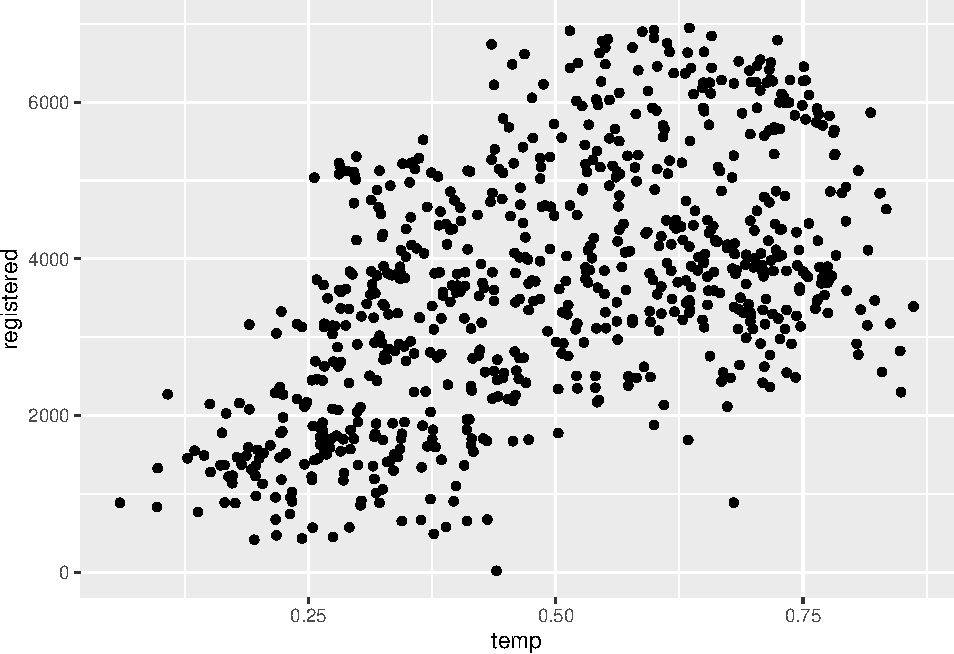
\includegraphics[width=0.5\linewidth]{rj-paper_files/figure-latex/int-pairs-bike-1} 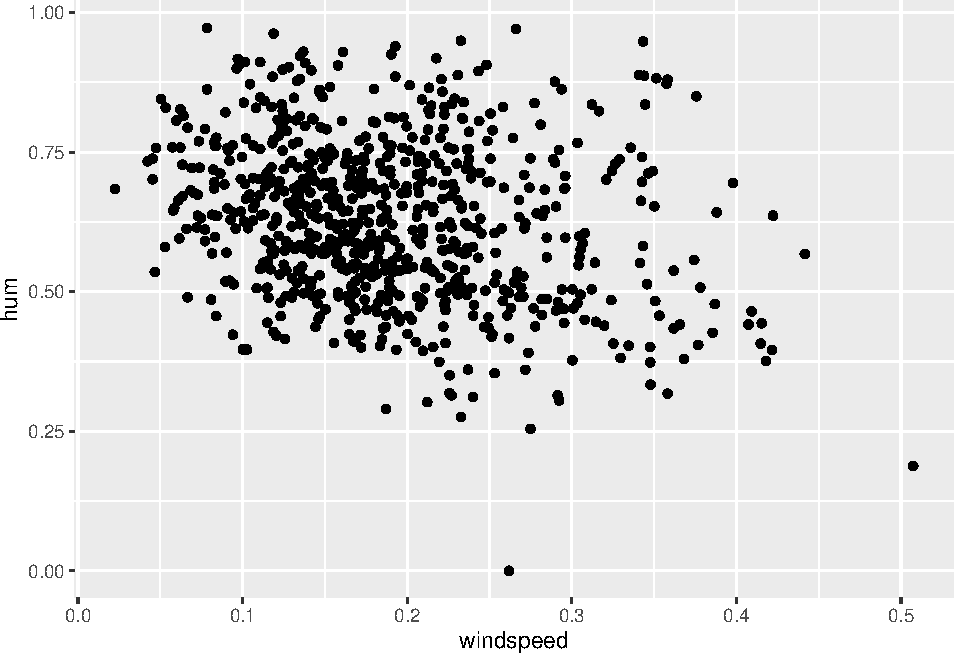
\includegraphics[width=0.5\linewidth]{rj-paper_files/figure-latex/int-pairs-bike-2} 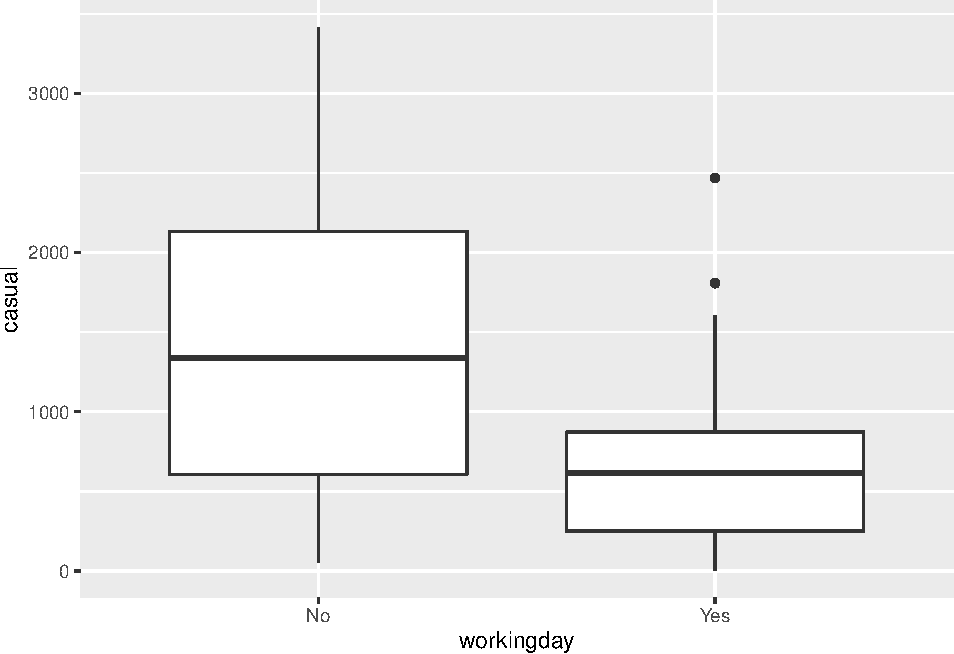
\includegraphics[width=0.5\linewidth]{rj-paper_files/figure-latex/int-pairs-bike-3} 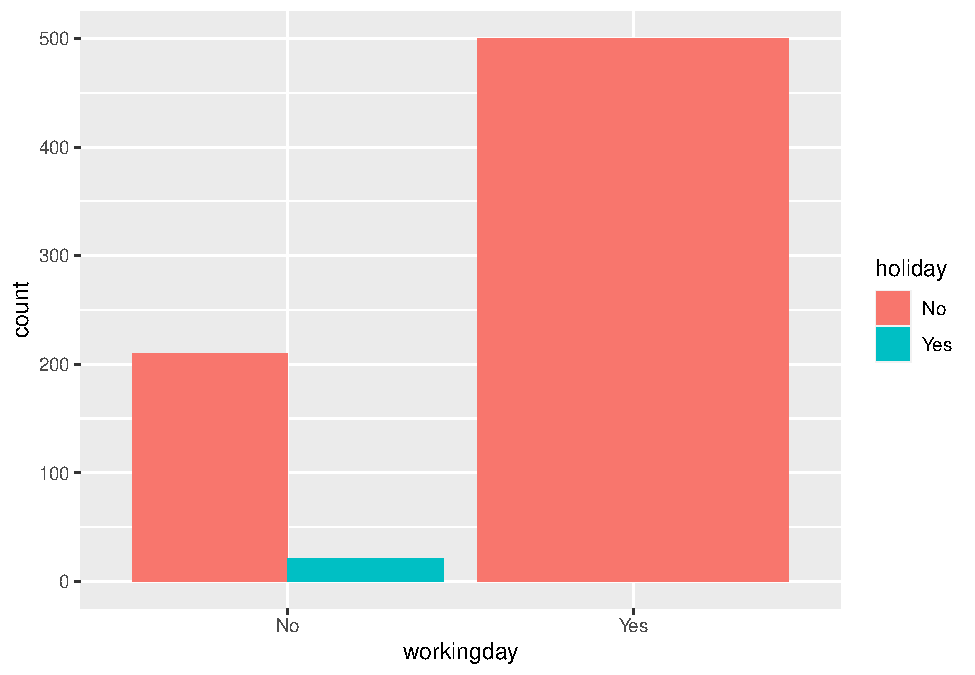
\includegraphics[width=0.5\linewidth]{rj-paper_files/figure-latex/int-pairs-bike-4} \caption{Scatterplots for numeric pair (temp,registered) and (windspeed,hum),  boxplot for mixed pair (workingday,casual) and barplot for ordinal pair ((workingday, holiday) showing association between the pairs of variables.}\label{fig:int-pairs-bike}
\end{figure}

\hypertarget{multiple-association-measures-plot}{%
\subsubsection{Multiple Association Measures Plot}\label{multiple-association-measures-plot}}

The multiple measures plot compares association measures for variable pairs in a dataset. This display is useful in detecting pairs showing non-linear association which then can be explored further in more detail. The first step in producing the display is to calculate multiple pairwise association measures for a dataset using the \texttt{calc\_assoc\_all} function. The \texttt{multi\_pairwise} output of the function is then fed into \texttt{plot\_assoc\_matrix} to produce a multiple measures display. The \texttt{plot\_assoc\_matrix} function constructs a matrix display where the diagonal cells represent the variables and off-diagonal cells show variable pairs with multiple association measures as lollipops. The height and colour of the lollipops are mapped with the absolute value and by the type of association measure.

For the seriation of this display, a similarity matrix is first obtained by taking the maximum association measure value for a variable pair. This is followed by steps similar to the seriation of the matrix display discussed above. We also order multiple measure types in each cell of the multiple measures display. We use a simple sorting approach by ordering the measure types in decreasing order of their average measure value. This locates measure types with high average values at the start of each cell.

Figure \ref{fig:compare-matrix} shows a multiple association measures plot in matrix layout for bike sharing dataset. We convert the factor variable \texttt{mnth} into numeric and use only numeric variables to produce the display. The plot compares the absolute values of association measures such as \texttt{ace}, \texttt{cancor}, \texttt{dcor}, \texttt{kendall}, \texttt{mic}, \texttt{nmi}, \texttt{pearson} and \texttt{spearman} for every variable pair in the dataset.

\begin{verbatim}
biken <- bike |>
  mutate(mnth=as.numeric(mnth)) |>
  select(where(is.numeric))

biken_assoc_all <-calc_assoc_all(biken)
plot_assoc_matrix(biken_assoc_all) 
\end{verbatim}

\begin{figure}

{\centering 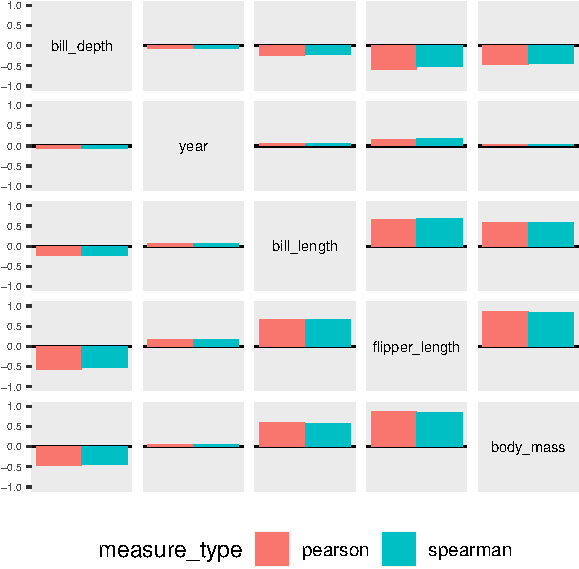
\includegraphics{rj-paper_files/figure-latex/compare-matrix-1} 

}

\caption{Seriated multiple association measures plot in a matrix layout for numeric variables in bike sharing data. The lollipops in each cell represent the value of the association measure colored by the type of measure. The variable pairs are ordered by the maximum value of association measures such that cells with highest value for any measure are close to the diagonal. The plot shows that pairs (casual,mnth) and (mnth,temp) might have a non-linear association which can be explored further.}\label{fig:compare-matrix}
\end{figure}

It is evident from the Figure \ref{fig:compare-matrix} that pairs (casual,mnth) and (mnth,temp) have higher value for \texttt{ace} compared to other measures. The measures \texttt{nmi}, \texttt{dcor} and \texttt{mic} have similar values but higher than \texttt{pearson}, \texttt{spearman} and \texttt{kendall}. This suggests the presence of a non-linear pattern for these pairs.

We use \texttt{show\_assoc} to explore the pattern for these variable pairs in Figure \ref{fig:int-pairs-multiple}. It is evident from the scatterplots that both (casual,mnth) and (mnth,temp) show a non-linear relationship which measures such as Pearson, Kendall or Spearman correlation failed to capture. The \texttt{ace} measure detects this non-linear association efficiently as the \texttt{ace} algorithm estimates the transformations of variables which leads to maximal correlation for the variable pair and uncovers non-linear pattern.

\begin{figure}
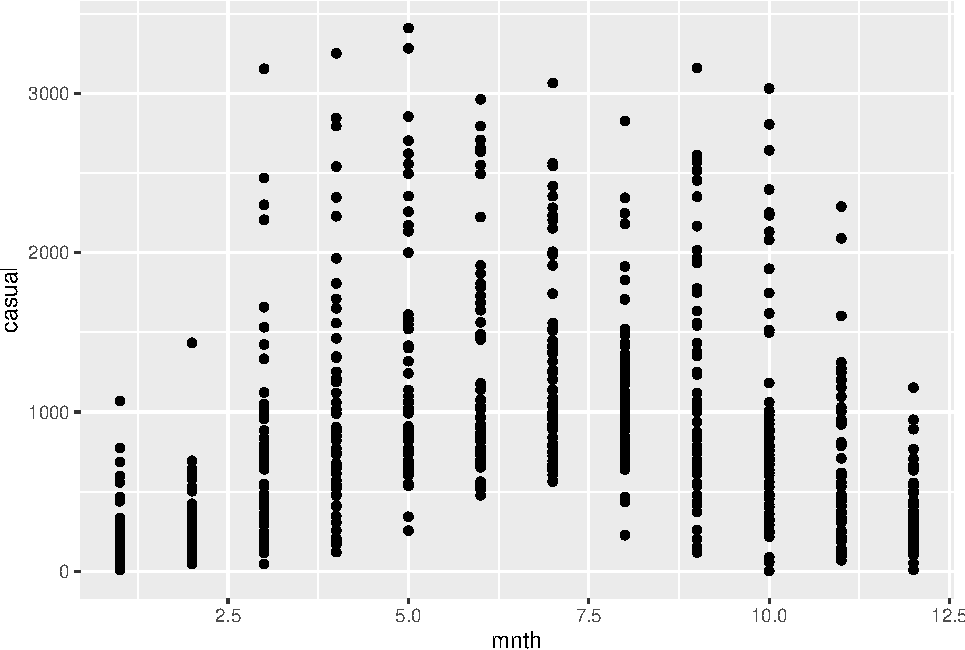
\includegraphics[width=0.5\linewidth]{rj-paper_files/figure-latex/int-pairs-multiple-1} 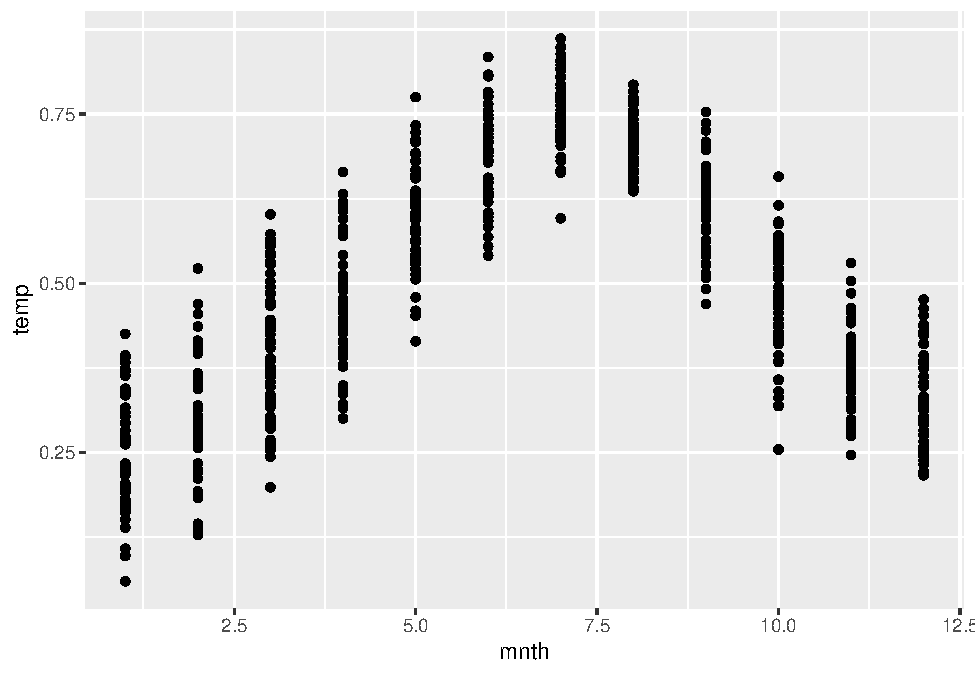
\includegraphics[width=0.5\linewidth]{rj-paper_files/figure-latex/int-pairs-multiple-2} \caption{Scatterplot for variable pairs (from left to right) (casual,mnth) and (mnth,temp) showing a non-linear relationship for these pairs.}\label{fig:int-pairs-multiple}
\end{figure}

\hypertarget{conditional-association-measures-plot}{%
\subsubsection{Conditional Association Measures Plot}\label{conditional-association-measures-plot}}

The conditional association measures plot explores bivariate association at different levels of a categorical variable. This display is useful for identifying pairs of variables showing different patterns at different levels of a grouping variable. To produce this display, the first step is to calculate association measures for the variable pairs using \texttt{calc\_assoc} function at each level of the grouping variable which is specified using the \texttt{by} argument. The \texttt{cond\_pairwise} output is then used as input to \texttt{plot\_assoc\_matrix} to produce a conditional measures display.

When supplied with \texttt{cond\_pairwise} object, the \texttt{plot\_assoc\_matrix} function constructs a conditional association measures display where the diagonal cells represent the variables and off-diagonal cells show variable pairs with association measures as lollipops for levels of a conditioning variable. The height and colour of the lollipops are mapped with the value of association measure and level of the conditioning variable respectively. The overall value of the association measure for the corresponding pair of variable in a cell is represented by a pink horizontal line.

For ordering the variables, we use a similar strategy as discussed above for matrix displays. The only difference is that a similarity matrix is constructed by taking the range of association measure values at different levels of the conditioning variable for a variable pair. For ordering levels of the conditioning variable in a cell, we follow a similar approach used for ordering measure types in multiple measures display.

Figure \ref{fig:cond-assoc} shows a conditional association plot for the bike sharing data in matrix layout. Each cell corresponding to a variable pair shows four lollipops which correspond to the association measure (Pearson's correlation for numeric pairs, Goodman and Kruskal's gamma for ordinal pair, canonical correlation for nominal or mixed pairs) calculated at the levels of conditioning variable \texttt{season}. The horizontal pink line represents the overall association measure for the pair. The plot shows a low overall correlation between hum and temp. This is also true in Spring and Winter, but the association is positive in fall and negative in Summer. Also, the overall correlation between registered and temp is moderate and positive. This is also true in each season except for summer where the correlation is about 0. The same pattern also holds for casual.

\begin{verbatim}
bike_by_assoc <- select(bike, -workingday, -holiday, -mnth, -yr) |>
  calc_assoc(by="season", 
                  coerce_types=list(ordinal=c( "weathersit")))


plot_assoc_matrix(bike_by_assoc)
\end{verbatim}

\begin{figure}

{\centering 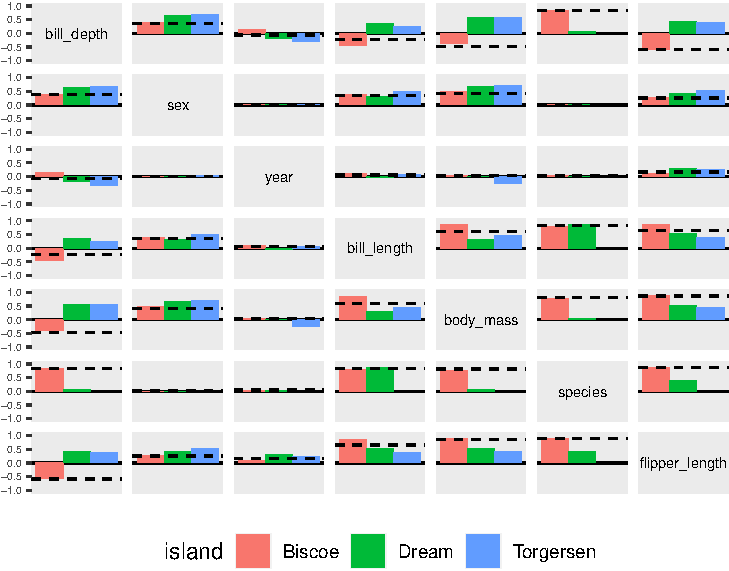
\includegraphics{rj-paper_files/figure-latex/cond-assoc-1} 

}

\caption{Seriated conditional association measures plot for bike sharing data showing Pearson's correlation for numeric pairs, Goodman and Kruskal's gamma for ordinal pair, canonical correlation for factor or mixed pairs. The lollipops in each cell represent the value for asssociation measure colored by the conditioning variable season. The pink horizontal line in each cell represents overall value of the association measure. The plot shows evident difference in measure value for pairs (temp, hum), (temp, registered), (temp, casual) and (registered, casual) for different seasons.}\label{fig:cond-assoc}
\end{figure}

We explore these variable pairs in more detail using \texttt{show\_assoc}. Figure \ref{fig:int-pairs-conditional} shows scatterplots for variable pairs (temp, hum), (temp, registered), (temp, casual) and (registered, casual) faceted by conditioning variable season. The faceted scatterplot for (temp, hum) show the decrease in humidity with increase in temperature in Summer and the oppsoite during Fall. Clearly, the plot for (temp, registered) and (temp, casual) show that there is no clear pattern for registered and casual with temperature in Summer compared to other seasons.

\begin{figure}
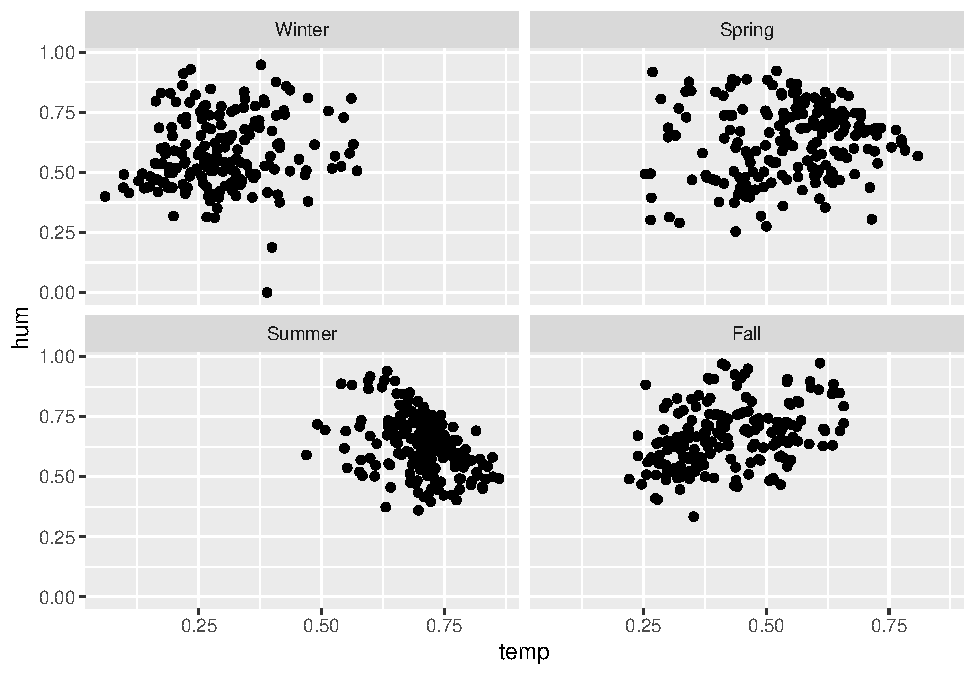
\includegraphics[width=0.5\linewidth]{rj-paper_files/figure-latex/int-pairs-conditional-1} 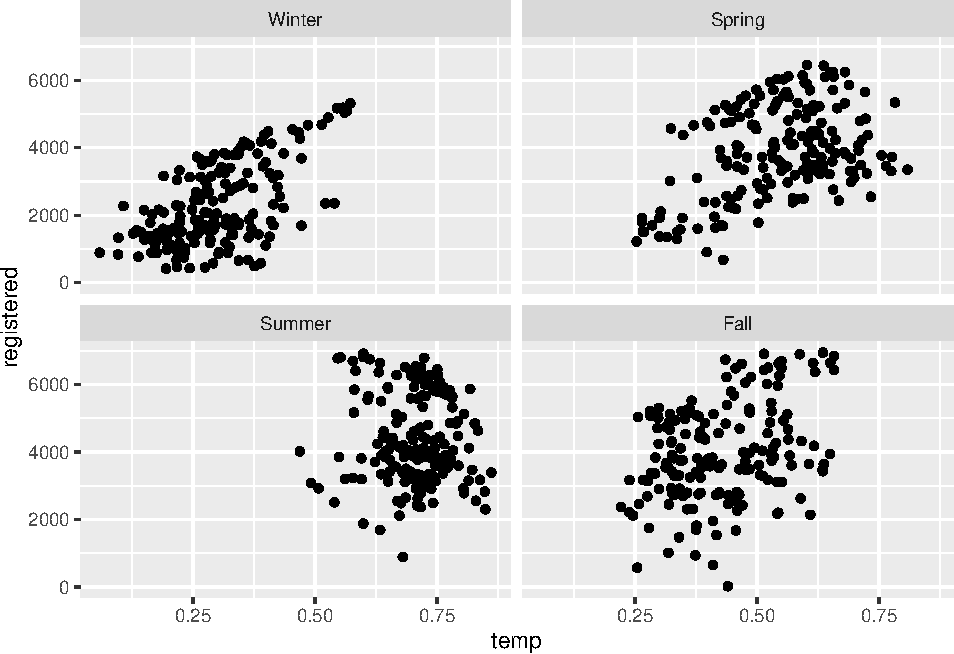
\includegraphics[width=0.5\linewidth]{rj-paper_files/figure-latex/int-pairs-conditional-2} 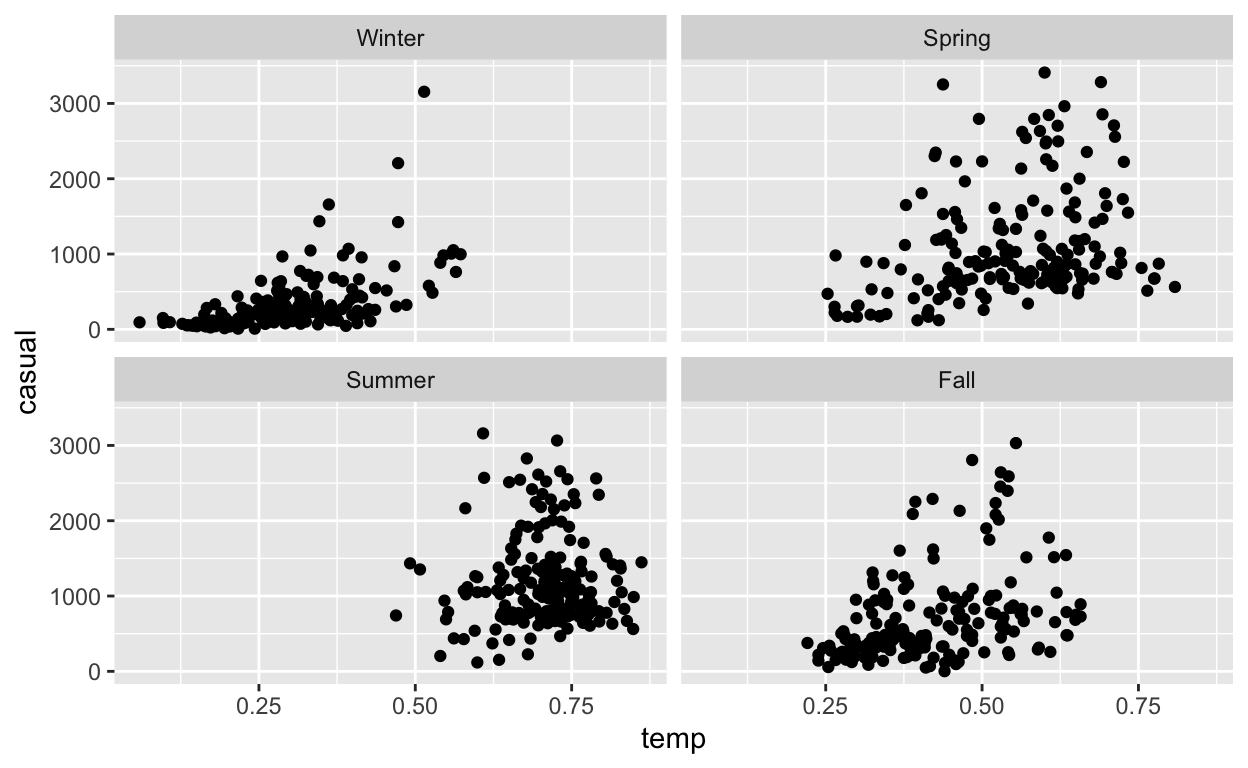
\includegraphics[width=0.5\linewidth]{rj-paper_files/figure-latex/int-pairs-conditional-3} 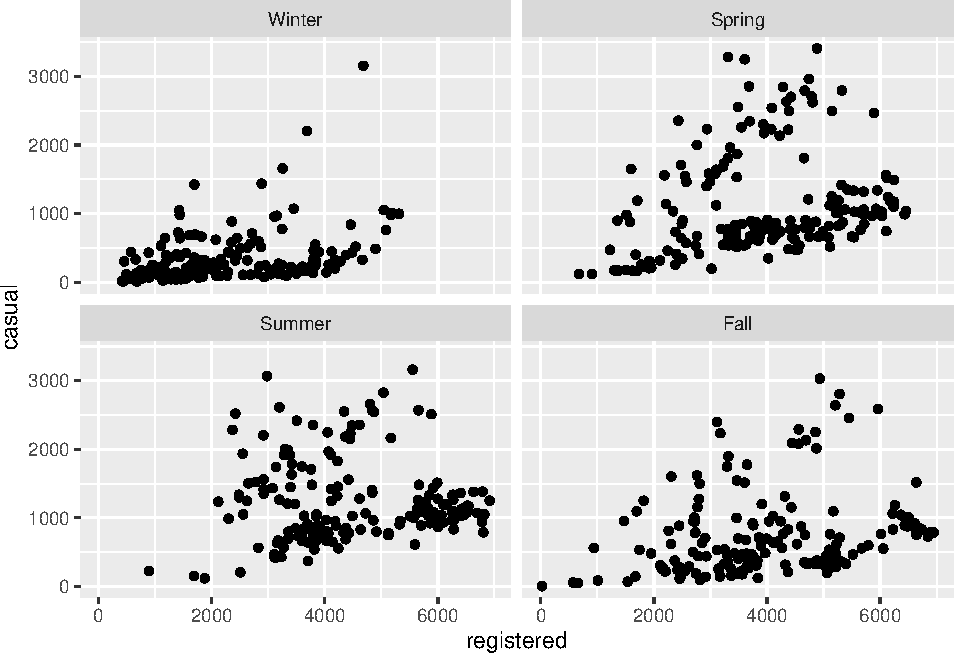
\includegraphics[width=0.5\linewidth]{rj-paper_files/figure-latex/int-pairs-conditional-4} \caption{Scatterplots for variable pairs (temp, hum), (temp, registered), (temp, casual) and (registered, casual) faceted by conditioning variable season}\label{fig:int-pairs-conditional}
\end{figure}

\hypertarget{linear-displays}{%
\subsection{Linear Displays}\label{linear-displays}}

We provide linear displays in the form of dot plots or heatmaps for plotting association measures and conditional association measures in \texttt{corVis}. These displays are handy for focusing on pairs of variables showing non-negligible associations. In \CRANpkg{corVis}, the \texttt{plot\_assoc\_linear} function constructs a plot in the linear layout displaying variable associations. The only required input for the \texttt{plot\_assoc\_linear} function is a data structure of class \texttt{pairwise}, \texttt{multi\_pairwise} or \texttt{cond\_pairwise}. We also provide importance sorting for these displays where the items ordered are variable pairs. We sort the variable pairs in decreasing order by either the maximum or the range between the measures for each pair.

Figure \ref{fig:linear-cond-assoc} shows a linear display for a \texttt{cond\_pairwise} data structure. The measures are displayed using dotplot (or a heatmap) where color of the dots (or each cell) is coded by the level of the partitioning variable. The plot shows filtered variable pairs having a difference in measure values equal to or greater than 0.25. It also shows Pearson's correlation for numeric pairs, Goodman and Kruskal's gamma for ordinal pairs and canonical correlation for factor or mixed pairs.

For ordering variable pairs of \texttt{cond\_pairwise} objects, we use the range of measures. The pairs of variables are ordered in descending order by range. As a result of this ordering, the variable pairs with the highest difference in measures are placed on the top of the display. This makes it easier to find triples of variables showing an interesting pattern. The pair of variables for which the measures at different levels are similar show that there is no effect of conditioning on their association.

Figure \ref{fig:linear-cond-assoc} shows that the variable pair (\texttt{hum}, \texttt{temp}) is placed at the top of the display and has the highest difference between the measures at different levels of \texttt{season}. The two variables humidity and temperature show opposite trends for the summer and fall seasons. This is expected as humidity generally decreases with temperature in summer whereas it tends to increase with temperature during the fall season.

\begin{verbatim}
bike_by_assoc <- select(bike, -workingday, -holiday, -mnth, -yr) |>
  calc_assoc(by="season", 
             coerce_types=list(ordinal=c( "weathersit")),
             include.overall = F)

bike_by_assoc |> 
  group_by(x,y) |> 
  summarise(range=max(measure,na.rm = T)-min(measure,na.rm = T)) |> 
  arrange(desc(range)) -> bike_by_assoc_rng
bike_by_assoc_rngf <- filter(bike_by_assoc_rng,range>=0.25) # filtering variable pairs with a range of 0.25 or greater
bike_by_assoc_mod <- filter(bike_by_assoc,
                          x %in% bike_by_assoc_rngf$x & y %in% bike_by_assoc_rngf$y)
plot_assoc_linear(bike_by_assoc_mod, 
                  plot_type = "dotplot",
                  pair_order = "max-min",
                  limits = c(-0.5,1))
\end{verbatim}

\begin{figure}

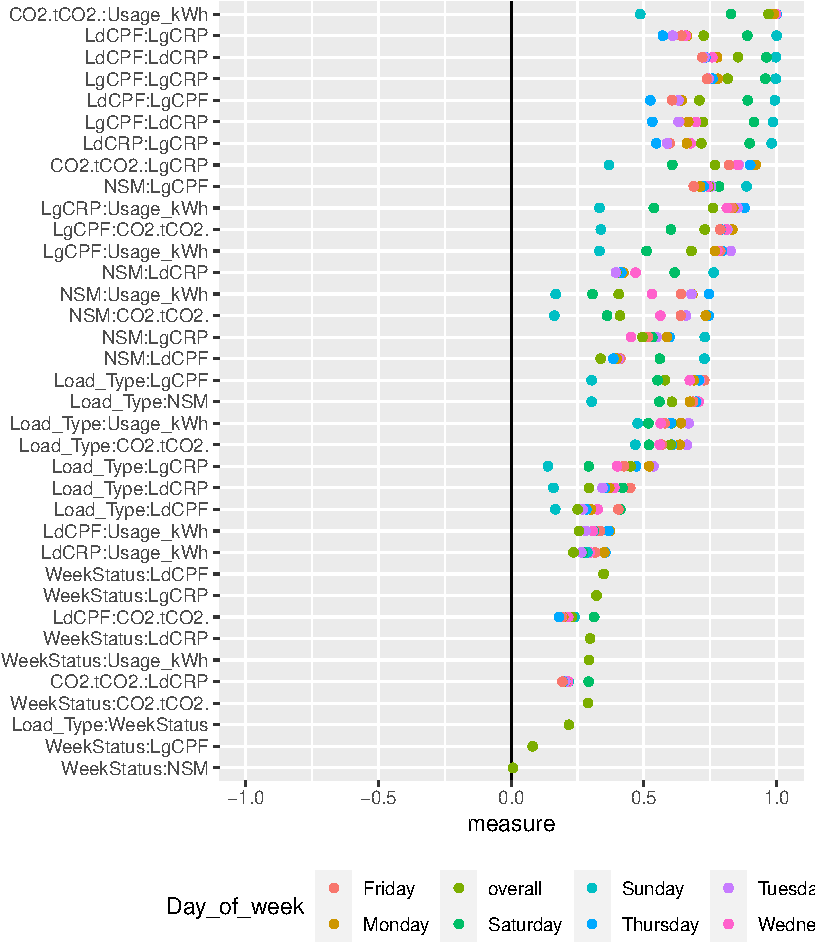
\includegraphics{rj-paper_files/figure-latex/linear-cond-assoc-1} \hfill{}

\caption{Conditional association measures plot for bike sharing data in linear layout.The display has variable pairs on the Y-axis and the value of association measures on the X-axis. The points corresponding to every variable pair represents the value of association measure for different levels of the conditioning variable and the overall value of association measure.}\label{fig:linear-cond-assoc}
\end{figure}

\hypertarget{discussion}{%
\section{Discussion}\label{discussion}}

We use multiple association measures in a single display for different variable pairs which serves as a comparison tool while exploring association in a dataset and assist in identifying unusual variable pairs. These multiple measures can be displayed in a scatterplot matrix similar to what Tukey and Tukey (1985) proposed. They suggested that scatterplot matrix of the scagnostics measures, which are measures summarizing a scatterplot, can be used to identify unusual scatterplots or variable pairs. Wilkinson, Anand, and Grossman (2005) used this idea with their graph-theoretic scagnostic measures to highlight unusual scatterplots. Similarly, (\textbf{kuhn2013applied?}) have used this idea in a predictive modeling context. They have produced a scatterplot matrix of the measures between the response and continuous predictors such as Pearson's correlation coefficient, pseudo-\(R^2\) from the locally weighted regression model, MIC and Spearman's rank correlation coefficient to explore the predictor importance during feature selection step. These displays show the importance of comparing multiple association measures at once for different variable pairs.

\hypertarget{references}{%
\section*{References}\label{references}}
\addcontentsline{toc}{section}{References}

\hypertarget{refs}{}
\begin{CSLReferences}{1}{0}
\leavevmode\vadjust pre{\hypertarget{ref-agresti2010analysis}{}}%
Agresti, Alan. 2010. \emph{Analysis of Ordinal Categorical Data}. Vol. 656. John Wiley \& Sons.

\leavevmode\vadjust pre{\hypertarget{ref-minerva}{}}%
Albanese, Davide, Michele Filosi, Roberto Visintainer, Samantha Riccadonna, Giuseppe Jurman, and Cesare Furlanello. 2012. {``Minerva and Minepy: A c Engine for the MINE Suite and Its r, Python and MATLAB Wrappers.''} \emph{Bioinformatics}, bts707.

\leavevmode\vadjust pre{\hypertarget{ref-DescTools}{}}%
Andri et mult. al., Signorell. 2022. \emph{{DescTools}: Tools for Descriptive Statistics}. \url{https://cran.r-project.org/package=DescTools}.

\leavevmode\vadjust pre{\hypertarget{ref-breiman1985estimating}{}}%
Breiman, Leo, and Jerome H Friedman. 1985. {``Estimating Optimal Transformations for Multiple Regression and Correlation.''} \emph{Journal of the American Statistical Association} 80 (391): 580--98.

\leavevmode\vadjust pre{\hypertarget{ref-timetk}{}}%
Dancho, Matt, and Davis Vaughan. 2022. \emph{Timetk: A Tool Kit for Working with Time Series in r}. \url{https://CRAN.R-project.org/package=timetk}.

\leavevmode\vadjust pre{\hypertarget{ref-bikeref}{}}%
Fanaee-T, Hadi, and Joao Gama. 2014. {``Event Labeling Combining Ensemble Detectors and Background Knowledge.''} \emph{Progress in Artificial Intelligence} 2: 113--27.

\leavevmode\vadjust pre{\hypertarget{ref-polycor}{}}%
Fox, John. 2022. \emph{Polycor: Polychoric and Polyserial Correlations}. \url{https://CRAN.R-project.org/package=polycor}.

\leavevmode\vadjust pre{\hypertarget{ref-friendly2002corrgrams}{}}%
Friendly, Michael. 2002. {``Corrgrams: Exploratory Displays for Correlation Matrices.''} \emph{The American Statistician} 56 (4): 316--24.

\leavevmode\vadjust pre{\hypertarget{ref-grimm2017kennzahlenbasierte}{}}%
Grimm, Katrin. 2017. {``Kennzahlenbasierte Grafikauswahl.''}

\leavevmode\vadjust pre{\hypertarget{ref-hills1969looking}{}}%
Hills, Michael. 1969. {``On Looking at Large Correlation Matrices.''} \emph{Biometrika} 56 (2): 249--53.

\leavevmode\vadjust pre{\hypertarget{ref-DendSer}{}}%
Hurley, Catherine B., and Denise Earle. 2022. \emph{DendSer: Dendrogram Seriation: Ordering for Visualisation}. \url{https://CRAN.R-project.org/package=DendSer}.

\leavevmode\vadjust pre{\hypertarget{ref-kendall1945treatment}{}}%
Kendall, Maurice G. 1945. {``The Treatment of Ties in Ranking Problems.''} \emph{Biometrika} 33 (3): 239--51.

\leavevmode\vadjust pre{\hypertarget{ref-kinney2014equitability}{}}%
Kinney, Justin B, and Gurinder S Atwal. 2014. {``Equitability, Mutual Information, and the Maximal Information Coefficient.''} \emph{Proceedings of the National Academy of Sciences} 111 (9): 3354--59.

\leavevmode\vadjust pre{\hypertarget{ref-corrr2020}{}}%
Kuhn, Max, Simon Jackson, and Jorge Cimentada. 2020. \emph{Corrr: Correlations in r}. \url{https://CRAN.R-project.org/package=corrr}.

\leavevmode\vadjust pre{\hypertarget{ref-corrgrapher}{}}%
Morgen, Pawel, and Przemyslaw Biecek. 2020. \emph{Corrgrapher: Explore Correlations Between Variables in a Machine Learning Model}. \url{https://CRAN.R-project.org/package=corrgrapher}.

\leavevmode\vadjust pre{\hypertarget{ref-murdoch1996graphical}{}}%
Murdoch, Duncan J, and ED Chow. 1996. {``A Graphical Display of Large Correlation Matrices.''} \emph{The American Statistician} 50 (2): 178--80.

\leavevmode\vadjust pre{\hypertarget{ref-olsson1979maximum}{}}%
Olsson, Ulf. 1979. {``Maximum Likelihood Estimation of the Polychoric Correlation Coefficient.''} \emph{Psychometrika} 44 (4): 443--60.

\leavevmode\vadjust pre{\hypertarget{ref-reshef2011detecting}{}}%
Reshef, David N, Yakir A Reshef, Hilary K Finucane, Sharon R Grossman, Gilean McVean, Peter J Turnbaugh, Eric S Lander, Michael Mitzenmacher, and Pardis C Sabeti. 2011. {``Detecting Novel Associations in Large Data Sets.''} \emph{Science} 334 (6062): 1518--24.

\leavevmode\vadjust pre{\hypertarget{ref-energy}{}}%
Rizzo, Maria, and Gabor Szekely. 2022. \emph{Energy: E-Statistics: Multivariate Inference via the Energy of Data}. \url{https://CRAN.R-project.org/package=energy}.

\leavevmode\vadjust pre{\hypertarget{ref-linkspotter}{}}%
Samba, Alassane. 2020. \emph{Linkspotter: Bivariate Correlations Calculation and Visualization}. \url{https://CRAN.R-project.org/package=linkspotter}.

\leavevmode\vadjust pre{\hypertarget{ref-commentSimonTibshirani}{}}%
Simon, Noah, and Robert Tibshirani. 2014. {``Comment on "Detecting Novel Associations in Large Data Sets" by Reshef Et Al, Science Dec 16, 2011.''} arXiv. \url{https://doi.org/10.48550/ARXIV.1401.7645}.

\leavevmode\vadjust pre{\hypertarget{ref-acepack}{}}%
Spector, Phil, Jerome Friedman, Robert Tibshirani, Thomas Lumley, Shawn Garbett, and Jonathan Baron. 2016. \emph{Acepack: ACE and AVAS for Selecting Multiple Regression Transformations}. \url{https://CRAN.R-project.org/package=acepack}.

\leavevmode\vadjust pre{\hypertarget{ref-speed2011correlation}{}}%
Speed, Terry. 2011. {``A Correlation for the 21st Century.''} \emph{Science} 334 (6062): 1502--3.

\leavevmode\vadjust pre{\hypertarget{ref-szekely2007measuring}{}}%
Székely, Gábor J, Maria L Rizzo, and Nail K Bakirov. 2007. {``Measuring and Testing Dependence by Correlation of Distances.''} \emph{The Annals of Statistics} 35 (6): 2769--94.

\leavevmode\vadjust pre{\hypertarget{ref-theil1970estimation}{}}%
Theil, Henri. 1970. {``On the Estimation of Relationships Involving Qualitative Variables.''} \emph{American Journal of Sociology} 76 (1): 103--54.

\leavevmode\vadjust pre{\hypertarget{ref-tukey1985computer}{}}%
Tukey, John W, and Paul A Tukey. 1985. {``Computer Graphics and Exploratory Data Analysis: An Introduction.''} In \emph{Proceedings of the Sixth Annual Conference and Exposition: Computer Graphics}, 85:773--85. 3.

\leavevmode\vadjust pre{\hypertarget{ref-corrplot2021}{}}%
Wei, Taiyun, and Viliam Simko. 2021. \emph{R Package 'Corrplot': Visualization of a Correlation Matrix}. \url{https://github.com/taiyun/corrplot}.

\leavevmode\vadjust pre{\hypertarget{ref-tidyverse}{}}%
Wickham, Hadley, Mara Averick, Jennifer Bryan, Winston Chang, Lucy D'Agostino McGowan, Romain François, Garrett Grolemund, et al. 2019. {``Welcome to the {tidyverse}.''} \emph{Journal of Open Source Software} 4 (43): 1686. \url{https://doi.org/10.21105/joss.01686}.

\leavevmode\vadjust pre{\hypertarget{ref-wilkinson2005graph}{}}%
Wilkinson, Leland, Anushka Anand, and Robert Grossman. 2005. {``Graph-Theoretic Scagnostics.''} In \emph{Information Visualization, IEEE Symposium on}, 21--21. IEEE Computer Society.

\end{CSLReferences}

\bibliography{RJreferences.bib}

\address{%
Amit Chinwan\\
Maynooth University\\%
Hamilton Institute\\ Maynooth, Ireland\\
%
%
%
\href{mailto:amit.chinwan.2019@mumail.ie}{\nolinkurl{amit.chinwan.2019@mumail.ie}}%
}

\address{%
Catherine Hurley\\
Maynooth University\\%
Department of Mathematics and Statistics\\ Maynooth, Ireland\\
%
%
%
\href{mailto:catherine.hurley@mu.ie}{\nolinkurl{catherine.hurley@mu.ie}}%
}
